% !TEX root = ./informe.tex

\section{Algoritmo Exacto}

\subsection{Explicación}

Nuestro problema a resolver es CFM: Clique de Frontera Máxima. Como aclaración, una clique es un subgrafo completo pero no necesariamente es maximal (aunque podría serlo). Debemos encontrar una clique en el grafo que tenga frontera máxima. Como una clique está formada por nodos del grafo, una forma de resolver CFM es revisando todos los posibles subconjuntos de nodos. En caso de que formen clique, calculamos su frontera y nos quedamos con el máximo de ellas.  \\

Para saber si un conjunto $vs$ de vértices es clique, revisamos si todos los vértices en $vs$ son vecinos entre sí. Esto significa que forman un subgrafo completo (pues los vértices y aristas forman parte del grafo principal) por lo tanto es clique. \\

Para calcular la frontera, dada una clique $c$ recorremos cada vértice $v \in c$ y contamos cuántos son los vecinos de $v$ que \textbf{no} están en $c$. \\

Si recorremos todos los subconjuntos posibles de nodos estamos recorriendo todas las posibles cliques, entonces podemos quedarnos con aquella que tenga máxima frontera. Siempre encuentra la solución óptima, pues encuentra todas las soluciones, implicando que efectivamente es un algoritmo exacto. \\

La implementación de la generación de todos los posibles subconjuntos está hecha recursivamente, utilizando el árbol binario que está implícito en la recursión. Considerando que cada nodo es un elemento, en cada etapa puede estar o no estar incluido, por lo que consideramos ambos estados posibles. Al final se terminan considerando todas las combinaciones posibles. \\

Una vez obtenido algún subconjunto (cuando ya no hay mas elementos que considerar), revisamos si lo acumulado forma clique, y en caso que sí, calculamos su frontera. Nos quedamos con la máxima de todas ellas. \\

\subsection{Pseudocódigo}

% (Ver notas debajo del pseudocodigo las referencia de significados de las variables)
Referencias de variables globales para el pseudocódigo:
\begin{itemize}
    \item $n$: La cantidad de nodos
    \item $solucion$: Secuencia que contiene la clique solución
    \item $fronteraMax$: El cardinal de la frontera de la clique solución
\end{itemize}

\begin{algorithm}[H]
\begin{algorithmic}
\Function{Resolver}{}
    \State LeerInput()                  \Comment $O(n^2)$
    \State $solucion \gets \emptyset$   \Comment $O(1)$
    \State $fronteraMax \gets 0$        \Comment $O(1)$
    \State GenerarSubconjuntos($\emptyset$, $0$) \Comment $O(2^{n} * n^{3})$
\EndFunction
\end{algorithmic}
\end{algorithm}

\begin{algorithm}[H]
\begin{algorithmic}
\Function{GenerarSubconjuntos}{$conjNodos$, $actual$} \Comment $O(2^{n} * n^{3})$, ver detalle en sección Complejidad.

    \If {$actual = n$}                  \Comment $O(1)$
        \If {EsClique($conjNodos$)}     \Comment $O(n^3)$
            \State $fronteraActual \gets$ Frontera($conjNodos$) \Comment $O(n^2)$
            \If {$fronteraActual > fronteraMax$}          \Comment $O(1)$
                \State $fronteraMax \gets fronteraActual$ \Comment $O(1)$
                \State $solucion \gets conjNodos$         \Comment $O(1)$
            \EndIf
        \EndIf

    \Else \Comment Ver sección Complejidad.
        \State GenerarSubconjuntos($conjNodos$, $actual + 1$)
        \State GenerarSubconjuntos($conjNodos \cup \{actual\}$, $actual + 1$)
    \EndIf
\EndFunction
\end{algorithmic}
\end{algorithm}

\begin{algorithm}[H]
\begin{algorithmic}
\Function{EsClique}{$conjNodos$}
    \For{$v \in conjNodos$}                     \Comment $O(n^3)$
        \For{$w \in conjNodos$}                 \Comment $O(n^2)$
            \If{$(v \neq w) \land (\neg$SonVecinos($v$, $w$)$)$}  \Comment $O(n)$
                \State return $False$                   \Comment $O(1)$
            \EndIf
        \EndFor
    \EndFor
    \State return $True$
\EndFunction
\end{algorithmic}
\end{algorithm}

\begin{algorithm}[H]
\begin{algorithmic}
\Function{SonVecinos}{$v1, v2$}
    \For{$w \in vecinos[v1]$}    \Comment $O(n)$
        \If{$w = v2$}            \Comment $O(1)$
            \State return $True$ \Comment $O(1)$
        \EndIf
    \EndFor
    \State return $False$        \Comment $O(1)$

\EndFunction
\end{algorithmic}
\end{algorithm}

\begin{algorithm}[H]
\begin{algorithmic}
\Function{Frontera}{$clique$}
    \State $enClique \gets vector(n, False)$ \Comment Vector con $n$ Falses, $O(n)$
    \For {$v \in clique$}                    \Comment $O(n)$
        \State $enClique[v] \gets True$      \Comment $O(1)$
    \EndFor

    \State $contador \gets 0$                \Comment $O(1)$
    \For{$v \in clique$}                     \Comment $O(n^2)$
        \For{$vecino \in vecinos[v]$}        \Comment $O(n)$
            \If{$\neg enClique[vecino]$}     \Comment $O(1)$
                \State $contador++$          \Comment $O(1)$
            \EndIf
        \EndFor
    \EndFor

    \State return $contador$                 \Comment $O(1)$

\EndFunction
\end{algorithmic}
\end{algorithm}

\subsection{Complejidad}

\begin{itemize}
    \item LeerInput es $O(n^2)$: Leo como máximo todas las aristas posibles.
    \item SonVecinos es $O(n)$: Recorro la lista de adyacencia de un vértice, como mucho tiene $O(n)$ vecinos.
    \item EsClique es $O(n^{3})$: Para cada vértice se recorren todos los demás y se revisa si son vecinos.
    \item Frontera es $O(n^{2})$: Para cada vértice de la clique se revisan todos sus vecinos.
    \item GenerarSubconjuntos es $O(2^{n} * n^{3})$: Hay $O(2^n)$ llamados recursivos (pues cada vértice está o no está), y en cada llamado recursivo se revisa si EsClique en $O(n^3)$ y luego su Frontera en $O(n^2)$ ($=$ $O(n^3)$). También puede pensarse que se generan $2^n$ subconjuntos, y por cada subconjunto se hacen $O(n^3)$ operaciones.
\end{itemize}

Para Resolver() se lee el input y luego se llama a GenerarSubconjuntos. La complejidad final es:

$$ O(n^2) + O(2^{n} * n^{3}) = O(2^{n} * n^{3})$$

\subsection{Experimentación}

Por lo que vimos en la sección complejidad, obtenemos la solución exacta pero a un costo temporal \textbf{muy} alto. Veamos empíricamente cuánto se tarda en resolver para cada tamaño de $n$. Consideramos para esta muestra grafos completos ya que tienen la máxima cantidad de vecinos por nodos, y son por lo tanto el peor caso. \\

Se puede observar en el siguiente gráfico cómo los tiempos aumentan exponencialmente con respecto al tamaño del grafo, y también puede observarse que para $n = 22$, se tardan aproximadamente 4 minutos. Es claro que es completamente inusable para grafos de mayor tamaño. \\

{\centering
    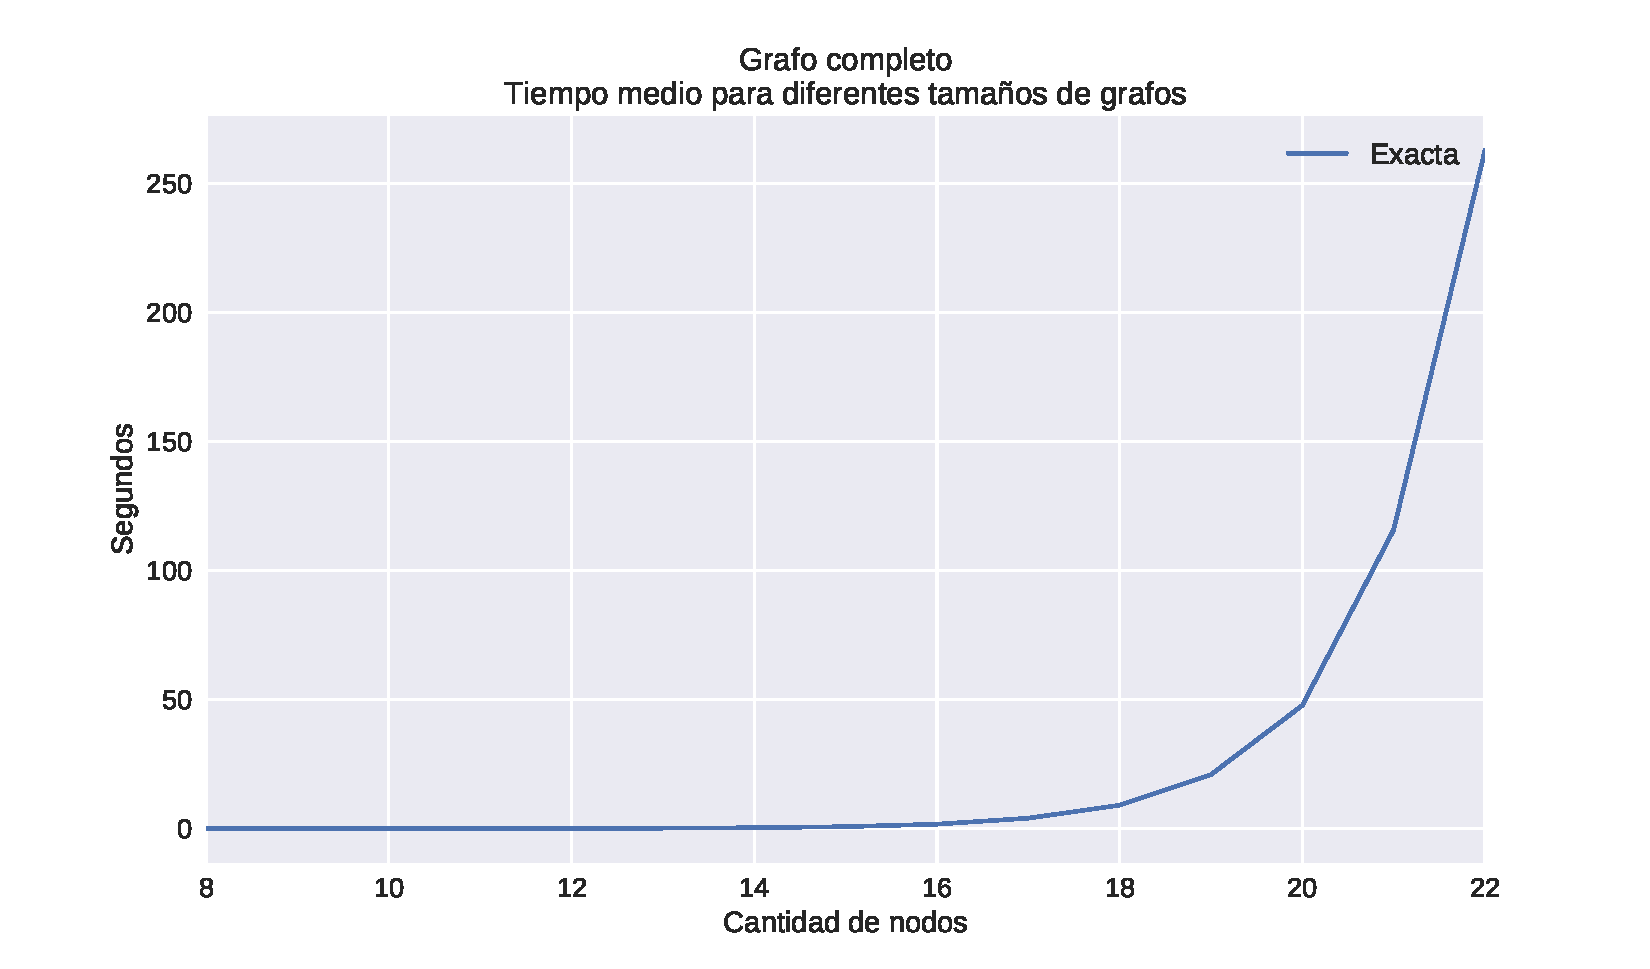
\includegraphics[width=1\textwidth]{informe/imgs/exp_completo_tiempo_exacta.pdf} \\
}

Aprovechemos esta sección para tratar de entender mejor el por qué de nuestras futuras estrategias. Una posible primera idea para encontrar la clique con máxima frontera es intentar encontrar la clique máxima. Esta es una \textit{pésima} idea, porque si consideramos un grafo completo de $n$ nodos, la clique máxima es $K_n$ con una frontera de tamaño 0. \\

Por ejemplo, vemos en el caso particular de los grafos completos que la clique que maximiza la frontera tiene tamaño $n/2$.

{\centering
    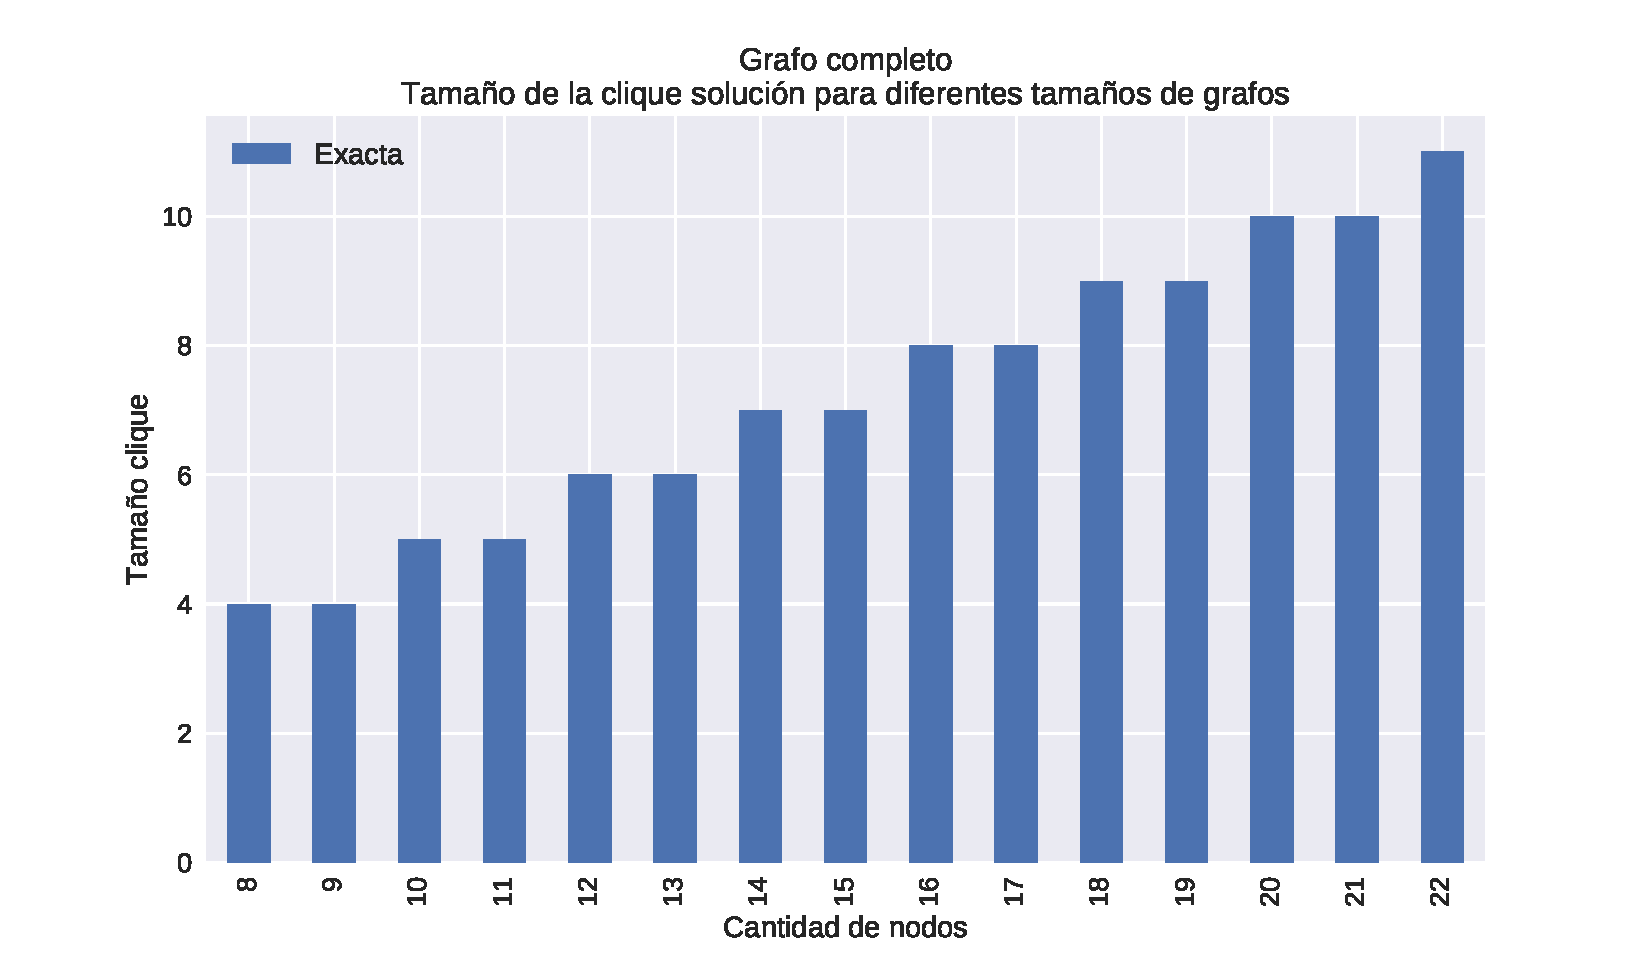
\includegraphics[width=1\textwidth]{informe/imgs/exp_completo_clique_exacta.pdf} \\
}

Como curiosidad, si nuestro grafo es completo no es necesario correr el algoritmo para conocer cuál será la frontera máxima. Basta considerar que la clique que la maximiza tiene $\frac{n}{2}$ nodos, y por cada nodo de la clique hay $\frac{n}{2}$ vecinos exteriores. Por lo tanto, la frontera máxima de un grafo completo es $\frac{n^2}{4}$.

% Not worthed
% {\centering
%     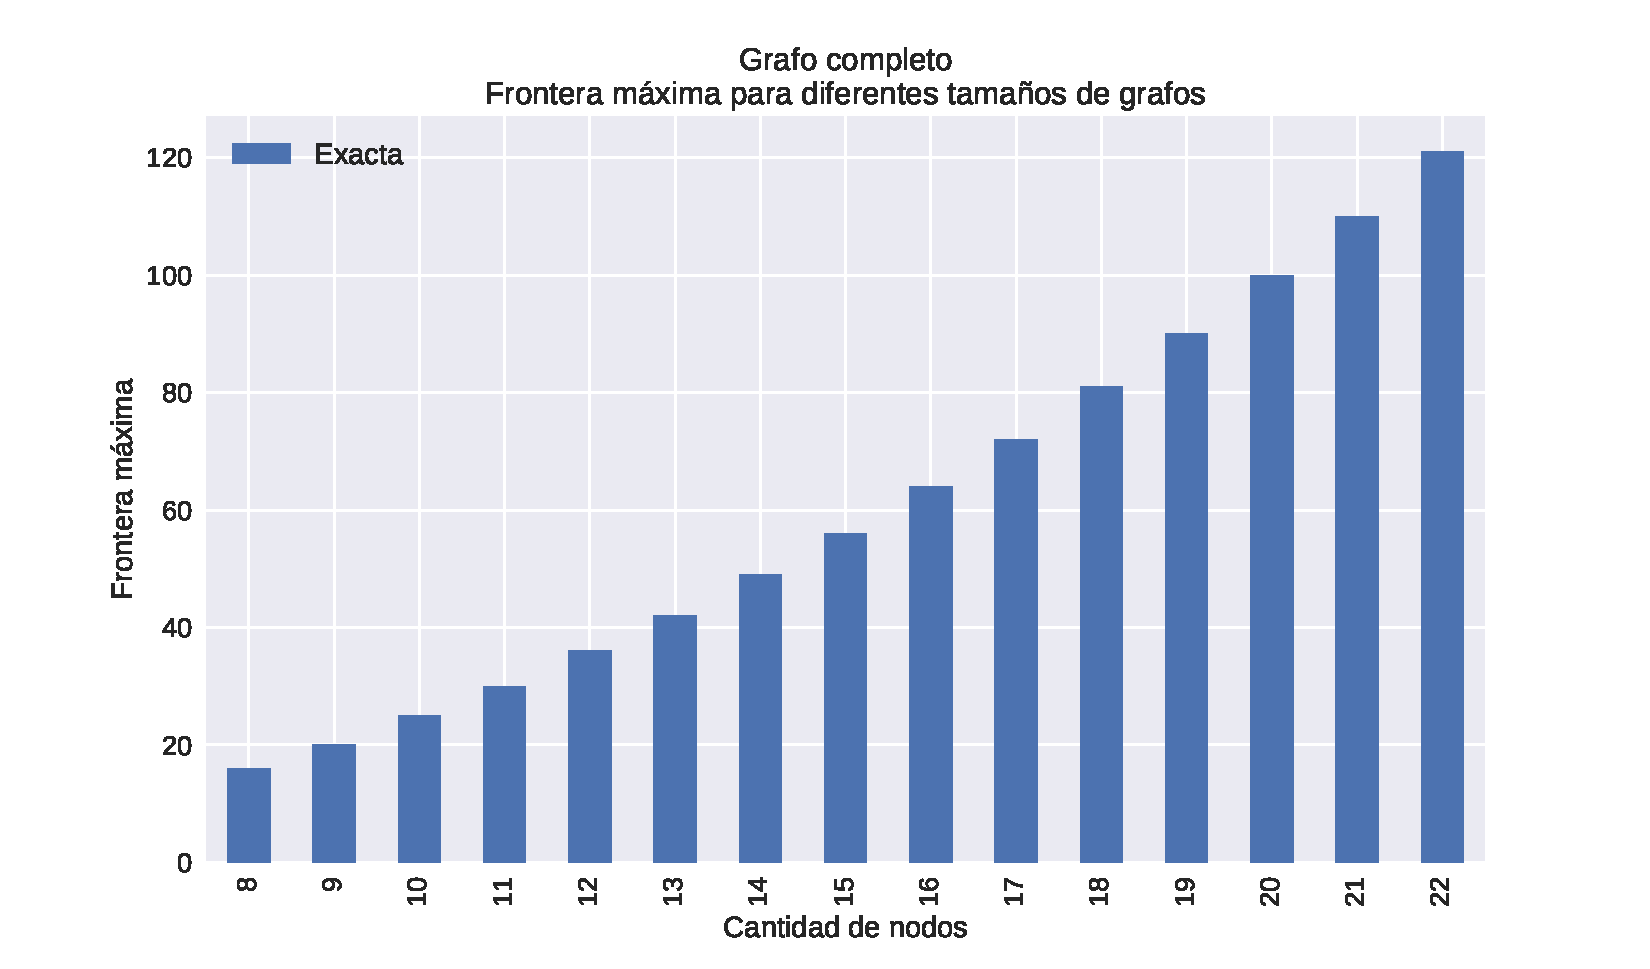
\includegraphics[width=1\textwidth]{informe/imgs/exp_completo_frontera_exacta.pdf} \\
% }

Si la clique es demasiado grande, es posible que disminuyamos la cantidad de vecinos que están fuera de la clique. Por lo tanto, la estrategia en las seguientes secciones no será buscar una clique máxima, sino ir construyéndolas pero solo mientras la frontera va aumentando. \\

Como vimos, esta forma de resolver el problema resulta impracticable. En las siguientes secciones analizaremos estrategias para poder resolverlo de formas mucho mas rápidas, pero a coste de no tener certeza de conseguir soluciones óptimas.
